
%% bare_conf.tex
%% V1.4b
%% 2015/08/26
%% by Michael Shell
%% See:
%% http://www.michaelshell.org/
%% for current contact information.
%%
%% This is a skeleton file demonstrating the use of IEEEtran.cls
%% (requires IEEEtran.cls version 1.8b or later) with an IEEE
%% conference paper.
%%
%% Support sites:
%% http://www.michaelshell.org/tex/ieeetran/
%% http://www.ctan.org/pkg/ieeetran
%% and
%% http://www.ieee.org/

%%*************************************************************************
%% Legal Notice:
%% This code is offered as-is without any warranty either expressed or
%% implied; without even the implied warranty of MERCHANTABILITY or
%% FITNESS FOR A PARTICULAR PURPOSE! 
%% User assumes all risk.
%% In no event shall the IEEE or any contributor to this code be liable for
%% any damages or losses, including, but not limited to, incidental,
%% consequential, or any other damages, resulting from the use or misuse
%% of any information contained here.
%%
%% All comments are the opinions of their respective authors and are not
%% necessarily endorsed by the IEEE.
%%
%% This work is distributed under the LaTeX Project Public License (LPPL)
%% ( http://www.latex-project.org/ ) version 1.3, and may be freely used,
%% distributed and modified. A copy of the LPPL, version 1.3, is included
%% in the base LaTeX documentation of all distributions of LaTeX released
%% 2003/12/01 or later.
%% Retain all contribution notices and credits.
%% ** Modified files should be clearly indicated as such, including  **
%% ** renaming them and changing author support contact information. **
%%*************************************************************************


% *** Authors should verify (and, if needed, correct) their LaTeX system  ***
% *** with the testflow diagnostic prior to trusting their LaTeX platform ***
% *** with production work. The IEEE's font choices and paper sizes can   ***
% *** trigger bugs that do not appear when using other class files.       ***                          ***
% The testflow support page is at:
% http://www.michaelshell.org/tex/testflow/





\documentclass[conference]{IEEEtran}
% Some Computer Society conferences also require the compsoc mode option,
% but others use the standard conference format.
%
% If IEEEtran.cls has not been installed into the LaTeX system files,
% manually specify the path to it like:
% \documentclass[conference]{../sty/IEEEtran}





% Some very useful LaTeX packages include:
% (uncomment the ones you want to load)


% *** MISC UTILITY PACKAGES ***
%
%\usepackage{ifpdf}
% Heiko Oberdiek's ifpdf.sty is very useful if you need conditional
% compilation based on whether the output is pdf or dvi.
% usage:
% \ifpdf
%   % pdf code
% \else
%   % dvi code
% \fi
% The latest version of ifpdf.sty can be obtained from:
% http://www.ctan.org/pkg/ifpdf
% Also, note that IEEEtran.cls V1.7 and later provides a builtin
% \ifCLASSINFOpdf conditional that works the same way.
% When switching from latex to pdflatex and vice-versa, the compiler may
% have to be run twice to clear warning/error messages.






% *** CITATION PACKAGES ***
%
\usepackage{cite}
% cite.sty was written by Donald Arseneau
% V1.6 and later of IEEEtran pre-defines the format of the cite.sty package
% \cite{} output to follow that of the IEEE. Loading the cite package will
% result in citation numbers being automatically sorted and properly
% "compressed/ranged". e.g., [1], [9], [2], [7], [5], [6] without using
% cite.sty will become [1], [2], [5]--[7], [9] using cite.sty. cite.sty's
% \cite will automatically add leading space, if needed. Use cite.sty's
% noadjust option (cite.sty V3.8 and later) if you want to turn this off
% such as if a citation ever needs to be enclosed in parenthesis.
% cite.sty is already installed on most LaTeX systems. Be sure and use
% version 5.0 (2009-03-20) and later if using hyperref.sty.
% The latest version can be obtained at:
% http://www.ctan.org/pkg/cite
% The documentation is contained in the cite.sty file itself.




%footnote package


\usepackage[vlined,ruled]{algorithm2e}






% *** GRAPHICS RELATED PACKAGES ***
%
\ifCLASSINFOpdf
   \usepackage[pdftex]{graphicx}
  % declare the path(s) where your graphic files are
  % \graphicspath{{../pdf/}{../jpeg/}}
  % and their extensions so you won't have to specify these with
  % every instance of \includegraphics
  % \DeclareGraphicsExtensions{.pdf,.jpeg,.png}
\else
  % or other class option (dvipsone, dvipdf, if not using dvips). graphicx
  % will default to the driver specified in the system graphics.cfg if no
  % driver is specified.
  % \usepackage[dvips]{graphicx}
  % declare the path(s) where your graphic files are
  % \graphicspath{{../eps/}}
  % and their extensions so you won't have to specify these with
  % every instance of \includegraphics
  % \DeclareGraphicsExtensions{.eps}
\fi
% graphicx was written by David Carlisle and Sebastian Rahtz. It is
% required if you want graphics, photos, etc. graphicx.sty is already
% installed on most LaTeX systems. The latest version and documentation
% can be obtained at: 
% http://www.ctan.org/pkg/graphicx
% Another good source of documentation is "Using Imported Graphics in
% LaTeX2e" by Keith Reckdahl which can be found at:
% http://www.ctan.org/pkg/epslatex
%
% latex, and pdflatex in dvi mode, support graphics in encapsulated
% postscript (.eps) format. pdflatex in pdf mode supports graphics
% in .pdf, .jpeg, .png and .mps (metapost) formats. Users should ensure
% that all non-photo figures use a vector format (.eps, .pdf, .mps) and
% not a bitmapped formats (.jpeg, .png). The IEEE frowns on bitmapped formats
% which can result in "jaggedy"/blurry rendering of lines and letters as
% well as large increases in file sizes.
%
% You can find documentation about the pdfTeX application at:
% http://www.tug.org/applications/pdftex





% *** MATH PACKAGES ***
%
\usepackage{amsmath}
% A popular package from the American Mathematical Society that provides
% many useful and powerful commands for dealing with mathematics.
%
% Note that the amsmath package sets \interdisplaylinepenalty to 10000
% thus preventing page breaks from occurring within multiline equations. Use:
%\interdisplaylinepenalty=2500
% after loading amsmath to restore such page breaks as IEEEtran.cls normally
% does. amsmath.sty is already installed on most LaTeX systems. The latest
% version and documentation can be obtained at:
% http://www.ctan.org/pkg/amsmath





% *** SPECIALIZED LIST PACKAGES ***
%
%\usepackage{algorithmic}
% algorithmic.sty was written by Peter Williams and Rogerio Brito.
% This package provides an algorithmic environment fo describing algorithms.
% You can use the algorithmic environment in-text or within a figure
% environment to provide for a floating algorithm. Do NOT use the algorithm
% floating environment provided by algorithm.sty (by the same authors) or
% algorithm2e.sty (by Christophe Fiorio) as the IEEE does not use dedicated
% algorithm float types and packages that provide these will not provide
% correct IEEE style captions. The latest version and documentation of
% algorithmic.sty can be obtained at:
% http://www.ctan.org/pkg/algorithms
% Also of interest may be the (relatively newer and more customizable)
% algorithmicx.sty package by Szasz Janos:
% http://www.ctan.org/pkg/algorithmicx




% *** ALIGNMENT PACKAGES ***
%
%\usepackage{array}
% Frank Mittelbach's and David Carlisle's array.sty patches and improves
% the standard LaTeX2e array and tabular environments to provide better
% appearance and additional user controls. As the default LaTeX2e table
% generation code is lacking to the point of almost being broken with
% respect to the quality of the end results, all users are strongly
% advised to use an enhanced (at the very least that provided by array.sty)
% set of table tools. array.sty is already installed on most systems. The
% latest version and documentation can be obtained at:
% http://www.ctan.org/pkg/array


% IEEEtran contains the IEEEeqnarray family of commands that can be used to
% generate multiline equations as well as matrices, tables, etc., of high
% quality.




% *** SUBFIGURE PACKAGES ***
%\ifCLASSOPTIONcompsoc
%  \usepackage[caption=false,font=normalsize,labelfont=sf,textfont=sf]{subfig}
%\else
%  \usepackage[caption=false,font=footnotesize]{subfig}
%\fi
% subfig.sty, written by Steven Douglas Cochran, is the modern replacement
% for subfigure.sty, the latter of which is no longer maintained and is
% incompatible with some LaTeX packages including fixltx2e. However,
% subfig.sty requires and automatically loads Axel Sommerfeldt's caption.sty
% which will override IEEEtran.cls' handling of captions and this will result
% in non-IEEE style figure/table captions. To prevent this problem, be sure
% and invoke subfig.sty's "caption=false" package option (available since
% subfig.sty version 1.3, 2005/06/28) as this is will preserve IEEEtran.cls
% handling of captions.
% Note that the Computer Society format requires a larger sans serif font
% than the serif footnote size font used in traditional IEEE formatting
% and thus the need to invoke different subfig.sty package options depending
% on whether compsoc mode has been enabled.
%
% The latest version and documentation of subfig.sty can be obtained at:
% http://www.ctan.org/pkg/subfig




 
 \usepackage[bottom]{footmisc}

% *** FLOAT PACKAGES ***
%
%\usepackage{fixltx2e}


% fixltx2e, the successor to the earlier fix2col.sty, was written by
% Frank Mittelbach and David Carlisle. This package corrects a few problems
% in the LaTeX2e kernel, the most notable of which is that in current
% LaTeX2e releases, the ordering of single and double column floats is not
% guaranteed to be preserved. Thus, an unpatched LaTeX2e can allow a
% single column figure to be placed prior to an earlier double column
% figure.
% Be aware that LaTeX2e kernels dated 2015 and later have fixltx2e.sty's
% corrections already built into the system in which case a warning will
% be issued if an attempt is made to load fixltx2e.sty as it is no longer
% needed.
% The latest version and documentation can be found at:
% http://www.ctan.org/pkg/fixltx2e


%\usepackage{stfloats}
% stfloats.sty was written by Sigitas Tolusis. This package gives LaTeX2e
% the ability to do double column floats at the bottom of the page as well
% as the top. (e.g., "\begin{figure*}[!b]" is not normally possible in
% LaTeX2e). It also provides a command:
%\fnbelowfloat
% to enable the placement of footnotes below bottom floats (the standard
% LaTeX2e kernel puts them above bottom floats). This is an invasive package
% which rewrites many portions of the LaTeX2e float routines. It may not work
% with other packages that modify the LaTeX2e float routines. The latest
% version and documentation can be obtained at:
% http://www.ctan.org/pkg/stfloats
% Do not use the stfloats baselinefloat ability as the IEEE does not allow
% \baselineskip to stretch. Authors submitting work to the IEEE should note
% that the IEEE rarely uses double column equations and that authors should try
% to avoid such use. Do not be tempted to use the cuted.sty or midfloat.sty
% packages (also by Sigitas Tolusis) as the IEEE does not format its papers in
% such ways.
% Do not attempt to use stfloats with fixltx2e as they are incompatible.
% Instead, use Morten Hogholm'a dblfloatfix which combines the features
% of both fixltx2e and stfloats:
%
% \usepackage{dblfloatfix}
% The latest version can be found at:
% http://www.ctan.org/pkg/dblfloatfix




% *** PDF, URL AND HYPERLINK PACKAGES ***
%
\usepackage{url}
% url.sty was written by Donald Arseneau. It provides better support for
% handling and breaking URLs. url.sty is already installed on most LaTeX
% systems. The latest version and documentation can be obtained at:
% http://www.ctan.org/pkg/url
% Basically, \url{my_url_here}.




% *** Do not adjust lengths that control margins, column widths, etc. ***
% *** Do not use packages that alter fonts (such as pslatex).         ***
% There should be no need to do such things with IEEEtran.cls V1.6 and later.
% (Unless specifically asked to do so by the journal or conference you plan
% to submit to, of course. )


% correct bad hyphenation here
%\hyphenation{op-tical net-works semi-conduc-tor}


\begin{document}
%
% paper title
% Titles are generally capitalized except for words such as a, an, and, as,
% at, but, by, for, in, nor, of, on, or, the, to and up, which are usually
% not capitalized unless they are the first or last word of the title.
% Linebreaks \\ can be used within to get better formatting as desired.
% Do not put math or special symbols in the title.
%\title{Towards a Provenance-Aware Internet of Things (IoT) System}

\title{Towards a Provenance Collection Framework for Internet of Things Devices }


% author names and affiliations
% use a multiple column layout for up to three different
% affiliations

%\author{\IEEEauthorblockN{Michael Shell}
%\IEEEauthorblockA{School of Electrical and\\Computer Engineering\\
%Georgia Institute of Technology\\
%Atlanta, Georgia 30332--0250\\
%Email: http://www.michaelshell.org/contact.html}
%\and
%\IEEEauthorblockN{Homer Simpson}
%\IEEEauthorblockA{Twentieth Century Fox\\
%Springfield, USA\\
%Email: homer@thesimpsons.com}
%\and
%\IEEEauthorblockN{James Kirk\\ and Montgomery Scott}
%\IEEEauthorblockA{Starfleet Academy\\
%San Francisco, California 96678--2391\\
%Telephone: (800) 555--1212\\
%Fax: (888) 555--1212}}

% conference papers do not typically use \thanks and this command
% is locked out in conference mode. If really needed, such as for
% the acknowledgment of grants, issue a \IEEEoverridecommandlockouts
% after \documentclass

% for over three affiliations, or if they all won't fit within the width
% of the page, use this alternative format:
% 
\author{\IEEEauthorblockN{
Ebelechukwu Nwafor,
Andre Campbell, 
David Hill,
 and
Gedare Bloom}
\IEEEauthorblockA{Department of Electrical Engineering and Computer Science\\
Howard University,
Washington, DC 20059\\ Email: ebelechukwu.nwafor@bison.howard.edu}
%\IEEEauthorblockA{\IEEEauthorrefmark{2}Twentieth Century Fox, Springfield, USA\\
%Email: homer@thesimpsons.com}
%\IEEEauthorblockA{\IEEEauthorrefmark{3}Starfleet Academy, San Francisco, California 96678-2391\\
%Telephone: (800) 555--1212, Fax: (888) 555--1212}
%\IEEEauthorblockA{\IEEEauthorrefmark{4}Tyrell Inc., 123 Replicant Street, Los Angeles, California 90210--4321}
}




%\author{\IEEEauthorblockN{Ebelechukwu Nwafor\IEEEauthorrefmark{1},
%Gedare Bloom\IEEEauthorrefmark{2}, Andre Campbell\IEEEauthorrefmark{3} and
%David Hill\IEEEauthorrefmark{4}}
%\IEEEauthorblockA{Department of Electrical Engineering and Computer Science\\
%\\ 2366 Sixth Street, NW, Washington, DC 20059\\
%Email: \IEEEauthorrefmark{1}ebelechukwu.nwafor@bison.howard.edu,
%\IEEEauthorrefmark{2}gedare@scs.howard.edu,
%\IEEEauthorrefmark{3}author.three@add.on.net,
%\IEEEauthorrefmark{4}author.four@add.on.net}}


% use for special paper notices
%\IEEEspecialpapernotice{(Invited Paper)}




% make the title area
\maketitle

% As a general rule, do not put math, special symbols or citations
% in the abstract
\begin{abstract}
The Internet of Things (IoT) offers immense benefits by enabling devices
to leverage networked resources thereby making intelligent decisions. The
numerous heterogeneous connected devices that exist throughout the IoT
system creates new security and privacy concerns. Some of these concerns
can be overcome through trust, transparency, and integrity, which can be
achieved with data provenance. Data provenance, also known as data lineage,
provides a history of transformations that occurs on a data object
from the time it was created to its current state. Data provenance has been
explored in the areas of scientific computing, business, forensic analysis, and
intrusion detection. Data provenance can help in detecting and mitigating
malicious cyber attacks. In this paper, we explore the integration of provenance within the IoT.
We introduce Provenance Aware Internet of Things System (PAIoTS), a  provenance collection framework for IoT devices. We evaluate the effectiveness
of our framework by looking at an application of provenance data by developing a prototype system for proof of concept.
\end{abstract}

% no keywords




% For peer review papers, you can put extra information on the cover
% page as needed:
% \ifCLASSOPTIONpeerreview
% \begin{center} \bfseries EDICS Category: 3-BBND \end{center}
% \fi
%
% For peerreview papers, this IEEEtran command inserts a page break and
% creates the second title. It will be ignored for other modes.
\IEEEpeerreviewmaketitle



\section{Introduction}
% no \IEEEPARstart
The Internet of Things (IoT) is transforming home, industrial and commercial automation exponentially and increasing the number of devices connected to the Internet. Cisco estimates that over 50 million devices will be connected to the internet by 2020 \cite{dave}. With the increasing amounts of connected heterogeneous devices, security and privacy risks also increase. For example, vulnerabilities in a brand of baby monitors allowed unauthorized access to devices whereby a malicious intruder can view live feeds from a remote location \cite{rapid7}. 

\par Due to the heterogeneity of devices and and the sensitivity of data generated on IoT devices, trust is a critical step to ensuring the security of IoT devices. This can be achieved through data provenance which is a comprehensive history of activities that occurred on an entity from its origin to its current state. Provenance ensures confidence in the fidelity of data. Provenance has been applied in domains such as scientific workflows for experiment reproducibility, information security as a form of access control, and also for intrusion detection. For IoT devices (things) that produce lots of sensor-actuator data, a workflow representation of sensor data can depict dependency between sensor readings and information stored or transmitted by the device. 

\par In this paper, we introduce Provenance Aware Internet of Things System (PAIoTS), a provenance collection framework for IoT devices, in which provenance data is collected and modeled to represent dependencies between sensor-actuator readings and IoT entities. Most of the interconnected heterogeneous devices are embedded systems that require lightweight and resource-efficient solutions as compared to general purpose
systems. This requirement is attributed to the constrained memory and computing power of such devices. We also contribute a provenance sensor model which provides a means to convert sensor event traces to provenance model graphs.



\section{Background} 
In this section, we  describe key concepts of data provenance, IoT characteristics, and provenance models. We also provide a smart home example for provenance collection in the IoT.

\subsection{Internet of Things}

In 1991, Mark Weiser, a pioneer of ubiquitous computing envisioned the notion of computing interleaved in our daily lives \cite{weiser1991}. Kevin Ashton, an early pioneer of IoT, defines the IoT as devices in our everyday lives which can be identified connected to a network \cite{ashton2009internet}. These devices can learn from information gathered autonomously without human input which allows for improvements in waste reduction and overall standard of living. Buckley et al. \cite{yan2008internet} define the IoT as a network of billions of machines communicating with each other. Gubbi et al \cite{gubbi_internet_2013} defines the IoT as an interconnection of sensing and actuating
devices that allows data sharing across platforms through a centralized framework. 

\par We define the IoT as a network of heterogeneous devices with sensing and actuating capabilities connected to internet-based cloud services. IoT has applications in home automation, smart health, automotive communication, machine to machine communication, industrial automation. Pervasive connectivity between heterogeneous devices allows them to share information with each other and with cloud based data analytics, which drives IoT. With analytics, IoT applications can learn from user data
to make smarter decisions. 



\par  IoT architecture represents a functional hierarchy of how information is disseminated across layers between devices which contain sensing and
actuating capabilities and massive data centers (cloud storage). Figure 1 displays the IoT architecture and the interactions between the respective
layers: sensor and actuator, device, gateway and cloud. The base of the architectural stack consists of sensors and actuators that gathers information from the physical world (via sensors) and manipulates it (via actuators) while interacting with the device layer. The device layer aggregates data from sensors and actuators and forwards the data to the gateway layer. The gateway layer routes and forwards this data collected from the
device layer to the cloud layer for storage and processing. Resource constraints decrease up the architectural stack, with
the cloud layer having the most resources (memory, power, computation), and the sensor-
actuator layer having the least. 


%\newtheorem{definition}{Definition}
%
%\begin{definition}
%
%The Internet of Things (IoT) is a network of heterogeneous devices with
%sensing and actuating capabilities communicating over the internet.
%
%\end{definition}


\begin{figure}[tb]
\begin{center}

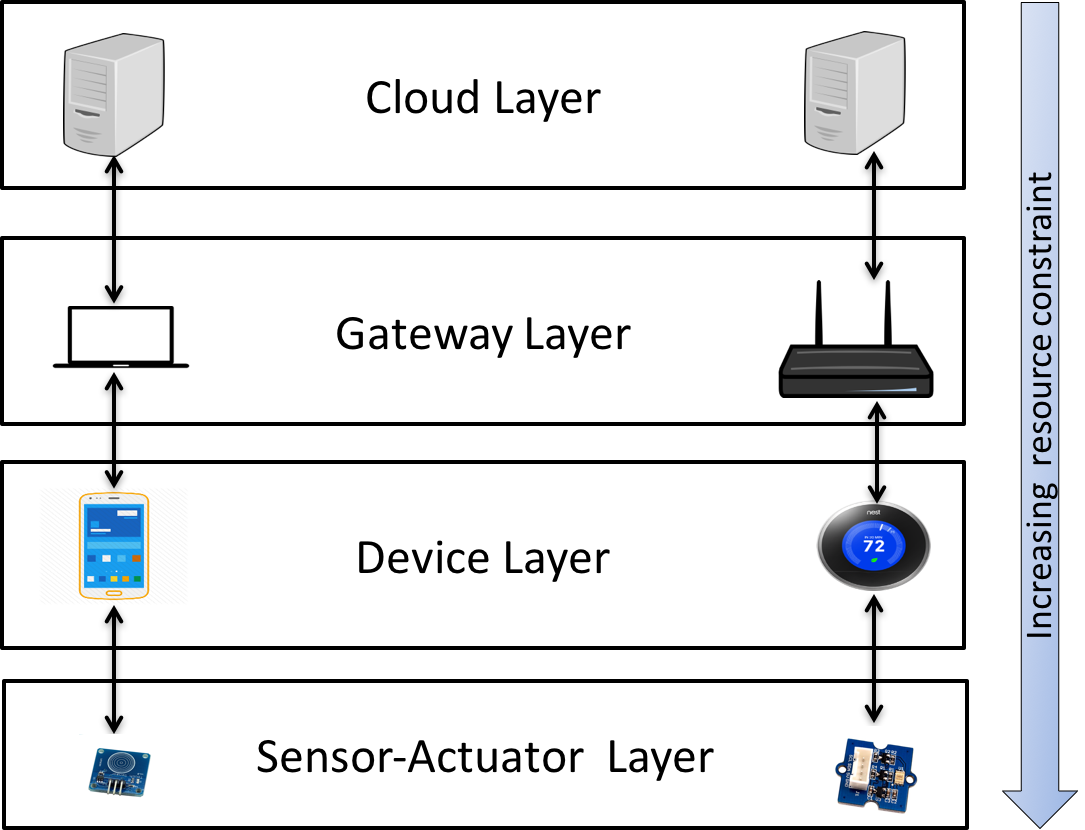
\includegraphics[height=2.0in]{iot_architecture.png}
\end{center}
\caption{IoT Architecture Diagram. The arrows illustrates the interaction between data at various layers on the architecture.}
\label{iot_architecture}

\end{figure}

\subsection{Motivating Use Case}

Creating a provenance collection system is beneficial to IoT because it
provides a means of verifying the integrity of data in the heterogeneous interconnected devices thereby building trust. Enabling provenance collection in IoT devices allows these devices to capture valuable information which enables backtracking in an event of a malicious attack. 


\begin{figure}[h!]
\begin{center}
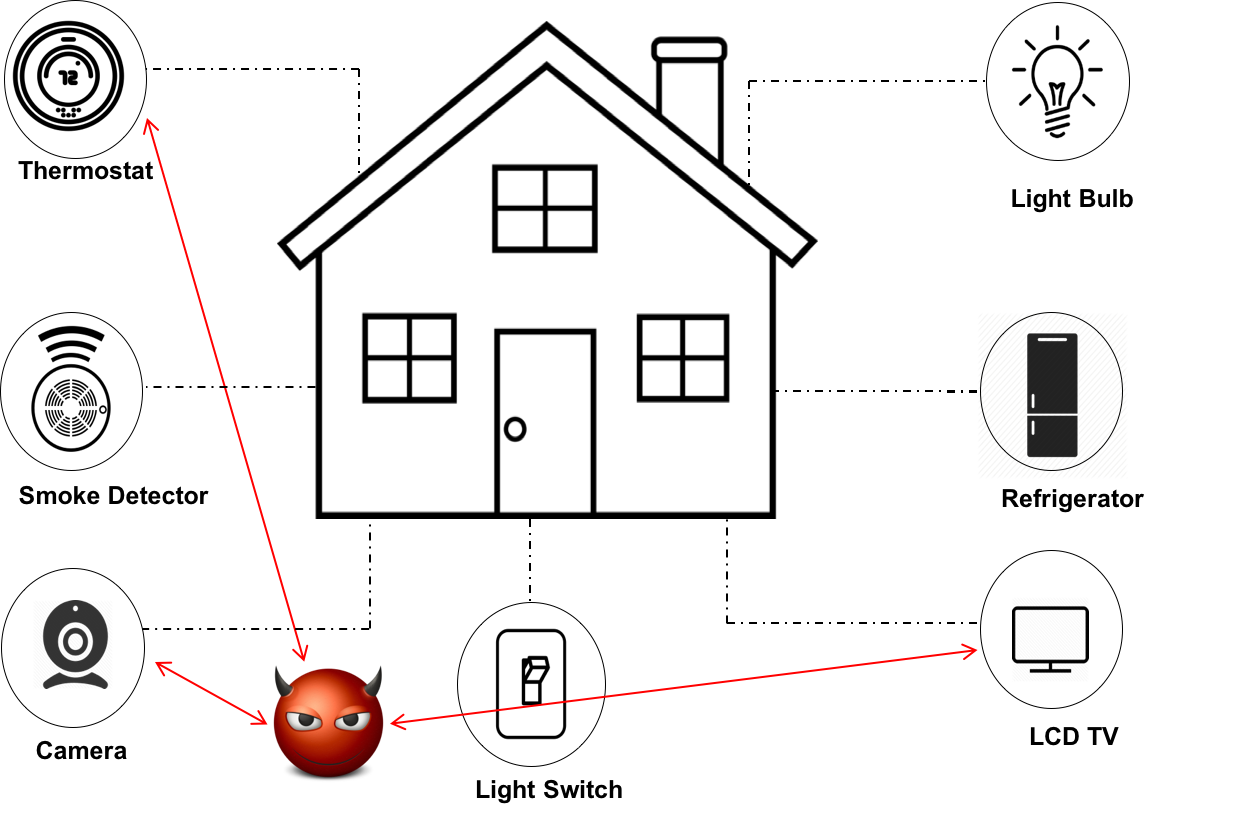
\includegraphics[height=2.5in]{smart_home.png}
\end{center}
\caption{Smart home use case scenario which demonstrates how provenance can be used to detect a point of entry of malicious intrusion}
\label{smart_home}
\end{figure}



Consider a smart home as illustrated in Figure \ref{smart_home} which contains interconnected devices such as a thermostat which automatically detects and regulates the temperature of a room based on prior information of a user's temperature preferences, a smart lock system that can be controlled remotely and informs a user via short messaging when the door has been opened, a home security camera monitoring system, a smart fridge which sends a reminder when food products are low etc. In an event that a malicious intruder attempts  to gain access to the security camera remotely, provenance information can be used to track the series  of events to determine where and how a malicious attack originated. Provenance can also be used as a safeguard to alert of a possible  compromise thereby protecting against future or ongoing attacks. 



\subsection{Data Provenance}

The Oxford English dictionary defines provenance as ``the place of origin or earliest
known history of something" \cite{TCDP1999}. An example of provenance can be seen with a college transcript. A transcript is the provenance of a college degree, because it identifies all of the
courses satisfied in order to attain the degree. In the field of computing, data provenance, also known as data lineage, is the history of all activities performed on an entity from its creation to its current state.
Cheney et al. \cite{cheney_provenance_2009}  describe provenance as the origin and history of data from its lifecycle. Buneman et al. \cite{buneman_why_2001} describe provenance from a database perspective as the origin of data and the steps in which it is derived in the database. We define data provenance of an entity as a comprehensive history of activities that occur on that entity from its creation to its present state.

%\begin{definition}
%Data provenance of an entity is a comprehensive history of activities that occur on that entity from its creation to its present state.
%\end{definition}

Provenance is easily represented as an acyclic graph which denotes causal relationships and dependencies between entities. Provenance consists of the following characteristics:
 
\begin{itemize}

\item Who: Provides information linking activities to an entity. Knowing the ``who" characteristic is essential because it maps the identity of modification to a particular data object. An example of ``who" in an IoT use case is a sensor device identifier.

\item Where: Location information at which data transformation was made. This provenance characteristic could be optional since not every data modification contains location details. An example is a GPS coordinate.

\item When: The time at which data transformation occurred. This is an essential provenance characteristic. Being able to tell the time of a data transformation allows for tracing data irregularities. An example of this characteristic is a timestamp that denotes when sensor data was read.

\item What: The transformation applied for example operations (create, read, update, and delete) that could be performed on a IoT data object.

\end{itemize}



%\subsubsection{Differentiating Provenance, Log data, and Metadata }
%
%Provenance has been used interchangably to define log data, and metadata. While some overlap exists between the three, some differences exist. Log data contains information about the activities of an operating system or processes. Log data might be used as provenance if it contains data trace specific to an application domain. Log files usually contain information such as error messages and warnings that might not be considered as provenance data. On the other hand, metadata contains descriptive information about data. Metadata can be considered as provenance when there exists a relationship between objects and they explain the transformation that occurs. In summary,  metadata and provenance are not the same, however an overlap exists. Metadata contains valuable  provenance information but not all metadata is provenance information. 


\subsection{Model for Representing Provenance for IoT}

%In order to represent provenance in an IoT architecture, we need to satisfy provenance characteristics (i.e who, where, when, and what of data transformations). 

Provenance of sensor readings in an IoT device should describe the dependency relationships between all entities responsible for producing those readings. We adopt the Provenance Data Model (PROV-DM) \cite{prov_dm}, a W3C standard which conforms to Provenance Ontology (PROV-O) and is used to depict dependencies between entities, activities and agents (digital or physical). PROV-DM creates a common model that allows for interchange of provenance information between heterogeneous devices and is represented serialized in three formats:  XML, JSON and RDF. 

\par PROV-DM contains two major components: types and relations.  Types can be entities, activities, or agents. An entity is a physical or digital object. An activity represents some form of action that occurs time.  An agent takes ownership of an entity, or performs an activity. Figure \ref{prov_rep} illustrates the types contained in PROV-DM and their graphical representation. Entities, activities and agents are represented by ovals, rectangles and hexagonals respectively. 


%We propose an alignment to the PROV-DM which contains information such as sensor readings, device name, and device information and give a detailed description of the alignment with use cases. Details on the provenance-sensor data model alignment is discussed in section IV.



\begin{figure}[h!]
\begin{center}

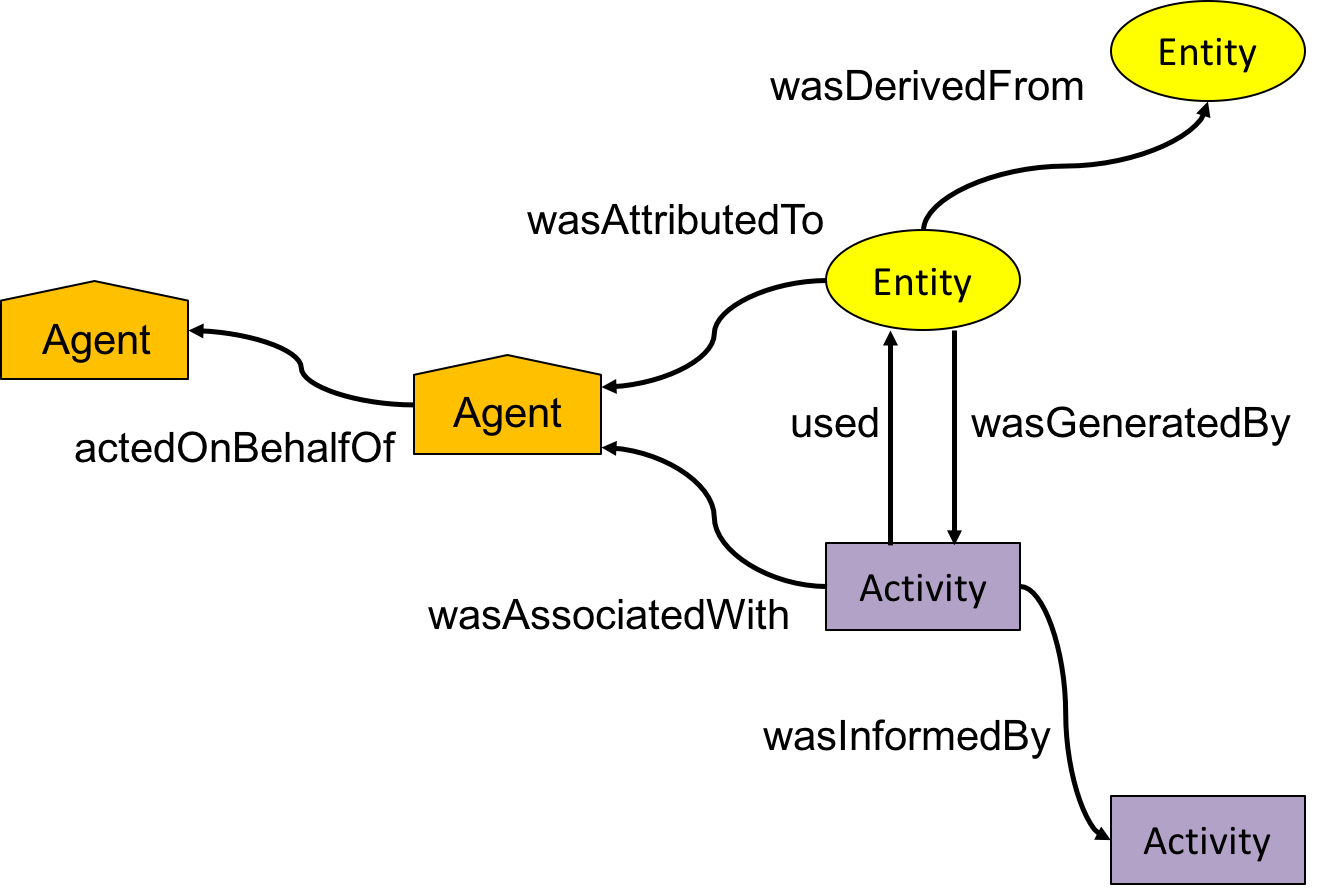
\includegraphics[width=3.0in]{prov_dm_2.PNG}
\end{center}
\caption{Prov-DM respresentation showing types in the model (Entity, Activity, and Agent) and the relationships between them }
\label{prov_rep}
\end{figure}


\par PROV-DM defines the following seven relationships between the types. 

\begin{itemize}
\item wasGeneratedBy:  Signifies the production of a new entity by an activity. 

\item used: An entity generated by one activity has been adopted by another activity.

\item wasInformedBy: Signifies the exchange of an entity by two activities.

\item wasDerivedFrom: Represents a copy of information from an entity. 

\item wasAttributedTo: Denotes relational dependency between an entity and an agent when the activity that created the agent is unknown.

\item wasAssociatedWith: An agent created or modified the activity

\item actedOnBehalfOf: Delegation of authority from an agent to itself or another agent to perform a particular responsibility. 



\end{itemize}



% An example of a floating figure using the graphicx package.
% Note that \label must occur AFTER (or within) \caption.
% For figures, \caption should occur after the \includegraphics.
% Note that IEEEtran v1.7 and later has special internal code that
% is designed to preserve the operation of \label within \caption
% even when the captionsoff option is in effect. However, because
% of issues like this, it may be the safest practice to put all your
% \label just after \caption rather than within \caption{}.
%
% Reminder: the "draftcls" or "draftclsnofoot", not "draft", class
% option should be used if it is desired that the figures are to be
% displayed while in draft mode.
%
%\begin{figure}[!t]
%\centering
%\includegraphics[width=2.5in]{myfigure}
% where an .eps filename suffix will be assumed under latex, 
% and a .pdf suffix will be assumed for pdflatex; or what has been declared
% via \DeclareGraphicsExtensions.
%\caption{Simulation results for the network.}
%\label{fig_sim}
%\end{figure}

% Note that the IEEE typically puts floats only at the top, even when this
% results in a large percentage of a column being occupied by floats.


% An example of a double column floating figure using two subfigures.
% (The subfig.sty package must be loaded for this to work.)
% The subfigure \label commands are set within each subfloat command,
% and the \label for the overall figure must come after \caption.
% \hfil is used as a separator to get equal spacing.
% Watch out that the combined width of all the subfigures on a 
% line do not exceed the text width or a line break will occur.
%
%\begin{figure*}[!t]
%\centering
%\subfloat[Case I]{\includegraphics[width=2.5in]{box}%
%\label{fig_first_case}}
%\hfil
%\subfloat[Case II]{\includegraphics[width=2.5in]{box}%
%\label{fig_second_case}}
%\caption{Simulation results for the network.}
%\label{fig_sim}
%\end{figure*}
%
% Note that often IEEE papers with subfigures do not employ subfigure
% captions (using the optional argument to \subfloat[]), but instead will
% reference/describe all of them (a), (b), etc., within the main caption.
% Be aware that for subfig.sty to generate the (a), (b), etc., subfigure
% labels, the optional argument to \subfloat must be present. If a
% subcaption is not desired, just leave its contents blank,
% e.g., \subfloat[].


% An example of a floating table. Note that, for IEEE style tables, the
% \caption command should come BEFORE the table and, given that table
% captions serve much like titles, are usually capitalized except for words
% such as a, an, and, as, at, but, by, for, in, nor, of, on, or, the, to
% and up, which are usually not capitalized unless they are the first or
% last word of the caption. Table text will default to \footnotesize as
% the IEEE normally uses this smaller font for tables.
% The \label must come after \caption as always.
%
%\begin{table}[!t]
%% increase table row spacing, adjust to taste
%\renewcommand{\arraystretch}{1.3}
% if using array.sty, it might be a good idea to tweak the value of
% \extrarowheight as needed to properly center the text within the cells
%\caption{An Example of a Table}
%\label{table_example}
%\centering
%% Some packages, such as MDW tools, offer better commands for making tables
%% than the plain LaTeX2e tabular which is used here.
%\begin{tabular}{|c||c|}
%\hline
%One & Two\\
%\hline
%Three & Four\\
%\hline
%\end{tabular}
%\end{table}


% Note that the IEEE does not put floats in the very first column
% - or typically anywhere on the first page for that matter. Also,
% in-text middle ("here") positioning is typically not used, but it
% is allowed and encouraged for Computer Society conferences (but
% not Computer Society journals). Most IEEE journals/conferences use
% top floats exclusively. 
% Note that, LaTeX2e, unlike IEEE journals/conferences, places
% footnotes above bottom floats. This can be corrected via the
% \fnbelowfloat command of the stfloats package.



%



\section {Provenance-Sensor Model}
In this section, we introduce the Provenance-Sensor Model and explain how PROV-O is used to convert sensor readings to provenance. Sensor data contains observation information such as temperature,and location details which can be transformed to standardized data interchange formats (RDF, XML, JSON). Sensor data are time series data which can be traced over time. Trace data containing sensor readings are important but do not depict dependency relationships when used alone. We transform trace data to provenance to represent causality and dependency relationships between entities in an IoT system. Provenance can be represented as a directed acyclic graph and the edge between two entities is considered a relation. Relations between data objects follows provenance ontology which depicts transformation between entities. We integrate PROV-O and sensor data for better representation of dependency relationships between trace data generated.

\par A single sensor might have the ability to collect multiple trace data, $td$. For example, a sensor might be able to collect sensor readings of temperature, location, humidity. A combination of trace data at a particular point in time is considered an event. We define an event  for sensor $s_1$ at time $t$ as $e= \{td_1, ...td_n\} $ where $td_1$ is the first trace data collected by $s_1$  and $td_n$ is the last which occurs at time $t$.





\par Adopting provenance ontology to IoT systems, we represent device information as agents (prov:agents), the operation performed on sensor readings (read, create, update) as a provenance activity (prov:activity), and events as entities (prov:entity). A sensor trace is defined as a tuple  $ (t, e, a, s_1, r_1)$ where $t$ represents a timestamp, $e$ an event, $a$ the operation, $s_1$ sensor information and $r_1$ device information.  


%\\ \\ $[s_1, r_1] \in \{prov:agent\}$  \\ $[e] \in \{prov:entity\} $ \\ $[a] \in \{prov:entity\}$ \\





\subsubsection{Device with to one sensor} 

Consider a humidity and temperature sensor $s_1$, connected to device $r_1$, a Raspberry Pi. Event $e= \{temperature, humidity\}$ therefore the tuple representation of trace data for sensor $s_1$ at time $t_1$ is $(t_1, \{temperature, humidity\}, a,  s_1, r_1)$. $a$ is the operation performed on the sensor. Each tuple is mapped to the Provenance Ontology representation using the defined constructs in section IV. Since $s_1$ is contained in device $r_1$, $r_1$ forms an edge with $s_1$ with the used relation. (e.g $r_1$ used $s_1$). 

\begin{figure}[h!]
\begin{center}

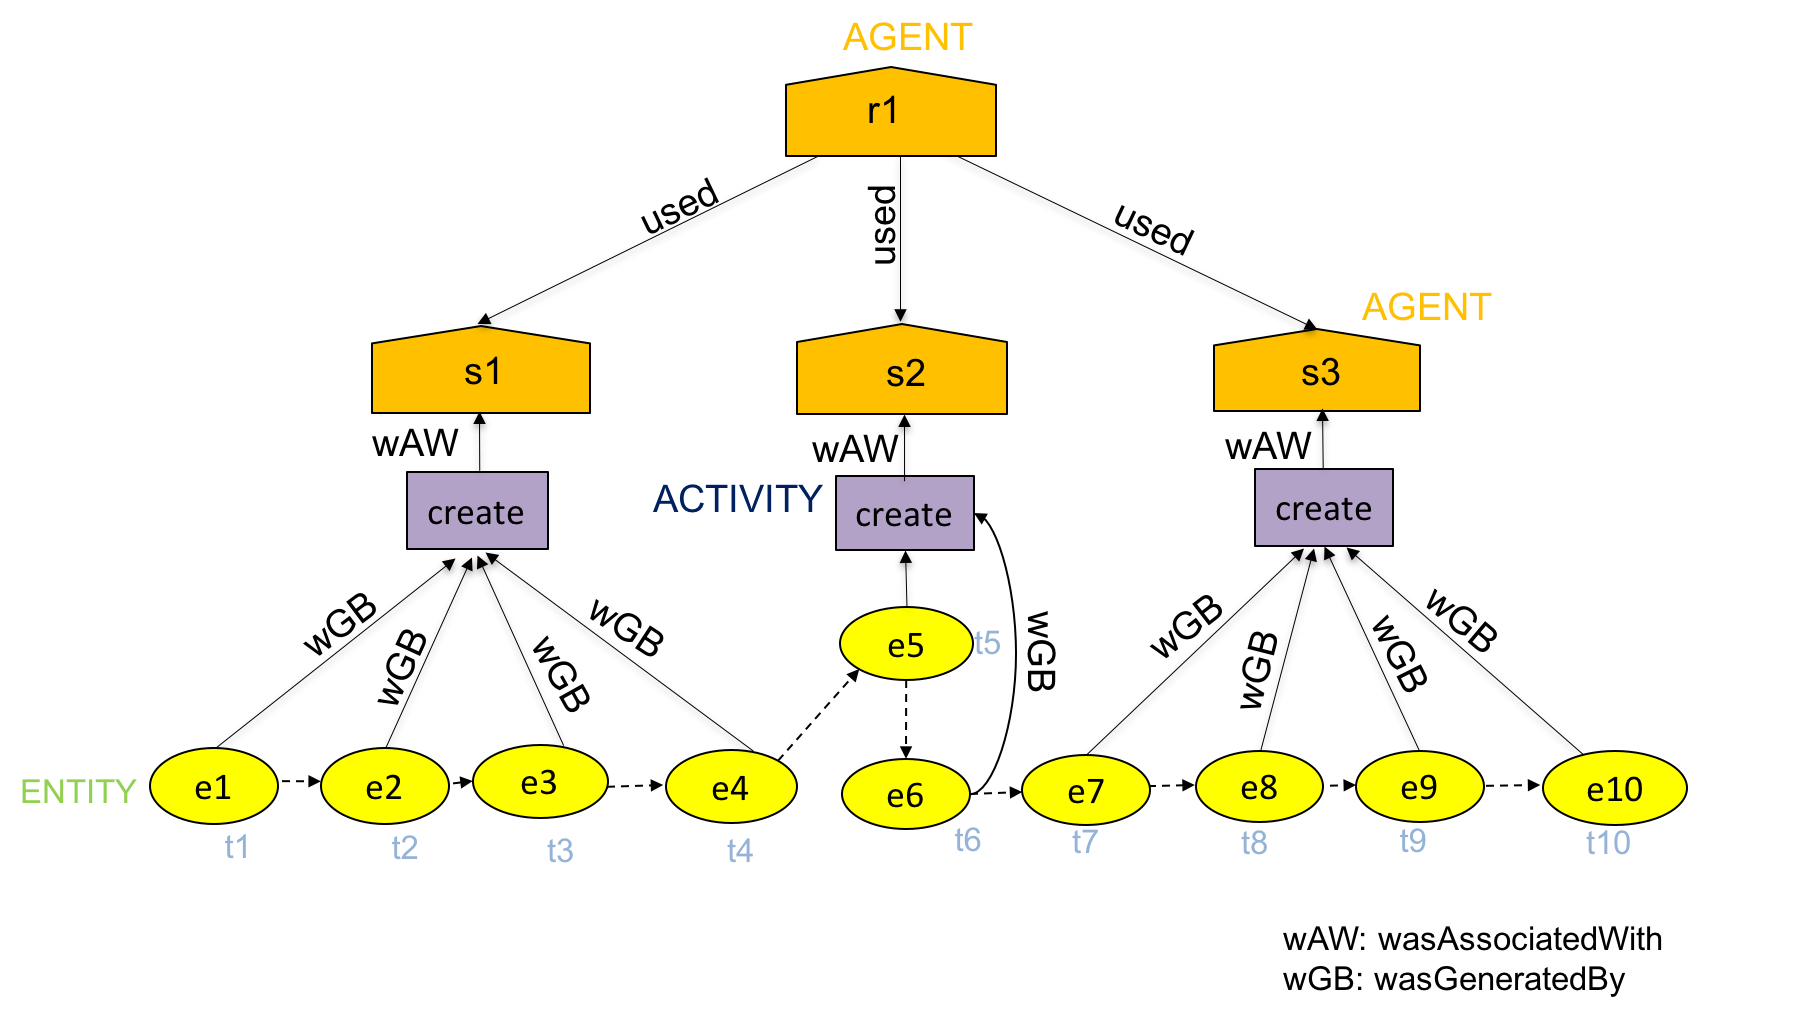
\includegraphics[width=3.8in]{prov_sensor_10.PNG}
\end{center}
\caption{Provenance-Sensor Model }
\label{prov_sensor}
\end{figure}

\subsubsection{Device with multiple sensors} 
Figure \ref{prov_sensor} further illustrates the concept of mapping provenance to sensor data using a graphical representation. The figure depicts a device connected to three sensors $s_1, s_2$, and $s_3$ with events  [$e_1, e_2,...,e_n$]. Data is generated by three identical temperature sensors, $s_1, s_2$ and $s_3$. The graph represents data dependency between $r_1$, the three sensors, the activity performed by the sensors (the sensors generate data in this case) and the events.  Each event makes an edge with the preceding event. Edges between events are denoted with a dotted arrow. This represents time dependency between events and that each events occur at different time. 


%The  graph of all of the events is:

% \\ For graph  G= (V, E):   \\ $V = \{ e_1, ...e_n \} \\  E = \{ (e_i,e_{i+1}): e_i, e_{i+1} \in V, e_1 \neq e_{i+1}\}  $ \\ 


%\( \\ G = (V, E) \\ V =  { e_1, ...e_n } \\ E = { (e_i,e_{i+1}): e_i, e_{i+1} \in V} \) 



\SetKwProg{Fn}{Function}{}{}


Algorithm \ref{Prov_sensor_alg} presents the steps taken by PAIoT to map sensor trace data into graph based provenance format. $F$  represents a  list of tuples $k$. For each tuples contained in F, $s, r_1$ represents sensor and device information respectively and are defined as agents. $e$ is defined as an event, $a$ is defined as an activity. $p$ is a memory representation of the provenance containing all  provenance types and their relations. x and y are a list of relations between sensor and device and activity and sensor, respectively.

\begin{algorithm}[h!]
\caption{Provenance-Sensor Mapping}
\label{Prov_sensor_alg}
\Fn{trace2Prov (F)}{

 p $\leftarrow$ createProvDocument() \\


\For{ k $\in$ F}{

\If{ s $\not\in$ p}{
s $\leftarrow$ createAgent() \\
}

\If{  $r_1 \not\in$ p}{
  $r_1 \leftarrow$ createAgent() \\
}
 
 e $\leftarrow$ createEntity()  \\

 a $\leftarrow$ createActivity() \\
 
 
 
 \If{ x $\not\in$ p}{
 
 x $\leftarrow$  relateSensorToDevice() \\
 
 }
 
\If{ y $\not\in$ p}{
 
 y $\leftarrow$ relateActivityToSensor()\\ 
 
 }
 
z $\leftarrow$ relateEntityToActivity()  \\
 
  

 
 
}

 return p \\
}

\end{algorithm}




\section{PAIoTS System Implementation}
In this section, we outline  PAIoTS, a trace-based provenance collection system for IoT devices. Figure \ref{architecture} displays the system architecture. Sensor readings in the form of input and output (I/O) events are recorded by the tracer component. This component intercepts I/O and produces trace information represented in Common Trace Format (CTF). 

%CTF encodes binary trace output information containing multiple streams of binary events such as I/O activity.

PAIoTS converts CTF trace data to provenance in our Provenance-Sensor Model. This conversion can happen at any layer of the IoT stack. CTF conversion to PROV-DM is done using babeltrace. Babeltrace is a plugin framework which allows the conversion of CTF traces into other formats. Trace or provenance data is securely transmitted to a gateway and later transmitted and stored in a cloud backend. Our backend of choice is Neo4j, a graph database with support for efficient storage, query and visualization of provenance data. 

\par CTF contains a mandatory stream known as metadata. Metadata contains information about other streams. It allows parsing a stream without specifying a layout. CTF encodes binary trace output information containing multiple streams of binary events such as I/O activity. Each event can be broken into streams. Streams allow for fast processing since they do not have to be stored in disk before being sent over a network or processed in memory.





\begin{figure}[h!]
\begin{center}

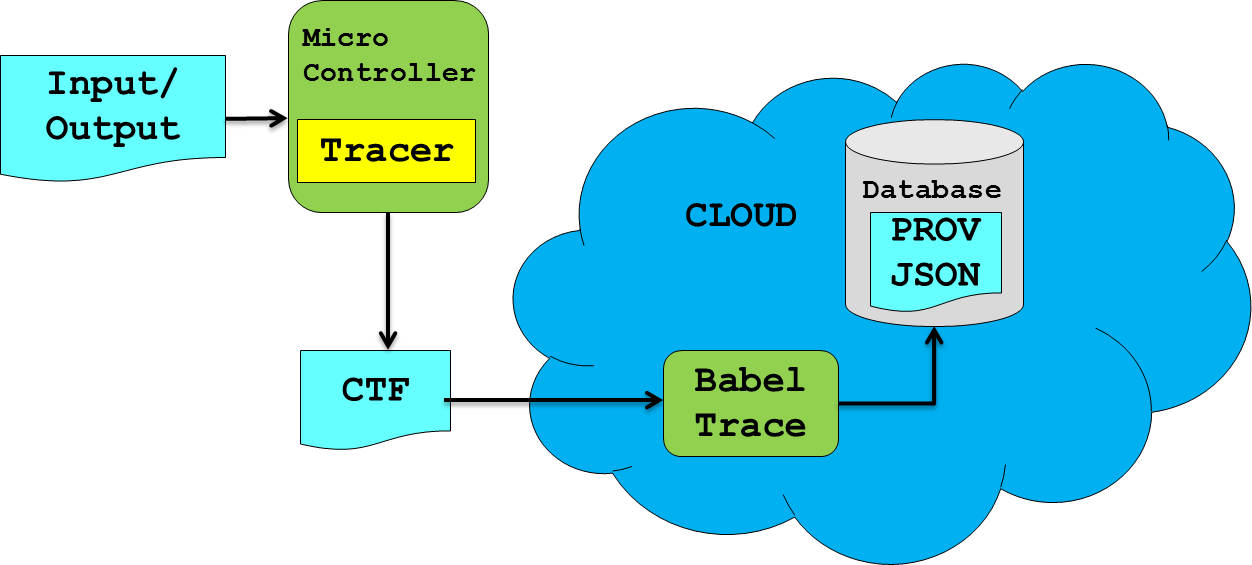
\includegraphics[width =3.0in]{system_architecture.PNG}    
\end{center}
\caption{System Architecture for PAIoTS.}
\label{architecture}
\end{figure}

Our provenance collection system records transformations of I/O data for devices connected in the IoT. For our implementation, we use several tools and hardware components in the development of our prototype:

\begin{itemize}
\item Raspberry Pi is the microcontroller used to demonstrate our approach. We chose Raspberry Pi because it is a representation of what can be found on an IoT gateway device. Raspberry Pi is a low cost, simple IoT demonstrator.

%\item Real Time Executive for Multiprocessor Systems (RTEMS) is an open source real­time operating system (RTOS) for embedded systems. This operating system is a typical RTOS that may be deployed in IoT devices.

\item Neo4j is a graph database which allows optimized querying of graph data such as provenance.

%\item lttng, a software tool for collecting system level trace on Linux system. 

\item Babeltrace is a trace converter tool to convert traces from one format into another. 

\item barectf is a light weight generator of C code  that generates trace data in CTF. 

\item  A yaml generator in barectf creates yaml  configuration files with information babeltrace needs to generate CTF trace output. Configuration  files contain settings such as an application trace stream, packet type, payload type and size. 

%\item rasberrypi

\end{itemize}

%\subsection{Prov-Aware IoT Information Flow }
%
%Place holder...
%
%\begin{figure}[h!]
%\begin{center}
%
%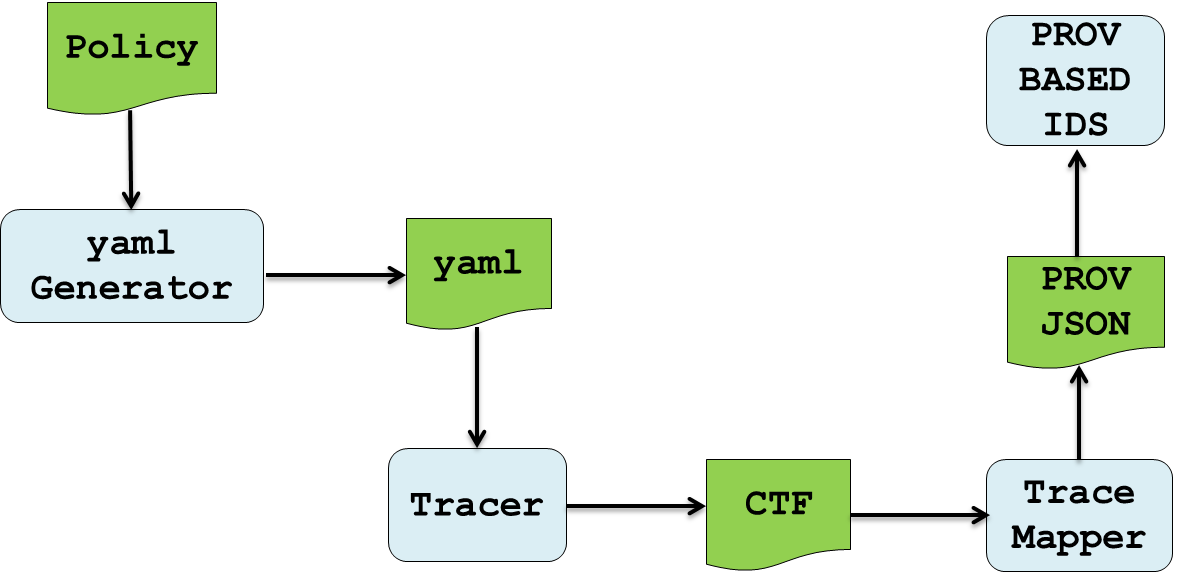
\includegraphics[width =3.0in]{flow.PNG}    
%\end{center}
%\caption{System Architecture for Provenance Collection.}
%\label{architecture}
%\end{figure}

%\section{Experiment}
%
%TODO...

\section{Related Work}

Muniswamy-Reddy
et al. \cite{muniswamy_reddy} developed Provenance Aware Storage System (PASS), a provenance collection system that tracks  system-level provenance of the Linux file system. Provenance information
is stored in the same location as the file system for easy accessibility, backup,
restoration, and data management. Provenance information is collected and stored in
the kernel space. PASS is composed of 3 major components: provenance collector, provenance storage, and provenance query. The collector keeps track of system level provenance. It intercepts system calls which are translated into provenance data and initially stored in memory. Provenance data is then transferred to a file system in an kernel database, BerkleyDB which maps key value pairs for provenance data for fast index look up. Our approach addresses application level provenance for memory constrained embedded systems. 

\par Bates et al. \cite{hi_fi}  developed, HiFi, a system level provenance collection framework for the Linux kernel using Linux Provenance Modules (LPM), which utilizes Linux Security Modules (LSM). LSM is a framework that was designed for providing custom access control inside the Linux kernel. HiFi contains three components: provenance collector, provenance log and provenance handler. The collector and log are contained in the kernel space while the handler is contained in the user space. The collector uses LSM to record provenance data and writes it to the provenance log. The handler reads the provenance record from the log. The log is a storage medium which transmits the provenance data to the user space. This approach to collecting provenance data differs from our work since we focus on memory constrained embedded systems which might not contain an operating system or a file system.

% Additionally,  HiFi deals with collecting system level events which might incur additional overhead when compared to collecting application level provenance. HiFi is engineered to work solely on the Linux operating system. Embedded systems that do not run on Linux OS will not be able to incorporate HiFi. 

\par RecProv \cite{rec_prov} is a provenance system which records user-level provenance, avoiding the overhead incurred by kernel level provenance recording. It does not require changes to the kernel like most provenance monitoring systems. It uses Mozilla rr to perform deterministic record and replay by monitoring system calls  and non deterministic input. The provenance information generated is converted into PROV-JSON, and stored in Neo4j, a graph database for visualization and storage of provenance graphs. In PAIoT, we convert trace data to provenance and also use Neo4j for storage and visualization of the provenance data however, our approach focuses on the relationship between entities in a device with limited computation and memory capabilities and also transformations of sensor data in these devices.



\par Spillance et al. \cite{story} developed a user space provenance collection system, Storybook that allows the use of application specific extensions such as database provenance, system level provenance, and web and email servers. Storybook captures provenance by intercepting system level events in the FUSE file system and storing in MySQL. StoryBook allows developers to implement provenance inspectors custom provenance models for specific applications which are often modified by different application (e.g web servers, databases). When an operation is performed on a data object, the appropriate provenance model is triggered and provenance data for that data object is captured. StoryBook stores provenance information such as open, close, read or write, application specific provenance, and causality relationship between entities contained in the provenance system. Provenance data is stored in key value pairs using Stasis and Berkely DB.  In our approach to provenance collection, we are particularly interested in the provenance of sensor data in memory constrained embedded systems.


%Collecting application level and kernel level events is similar to our approach of provenance collection, but 

\par Lim et al. \cite{lim} developed a
model for calculating the trust of nodes in a sensor network by using data
provenance and data similarity as deciding factors to calculate trust. The value of
provenance signifies that the more similar a data value is, the higher the trust score.
Also, the more the provenance of similar values differ, the higher their trust score. The trust score of a system is affected by the trust score of the sensor that forwards data to the system. Provenance is determined by the path data travels through the sensor network. This work differs from our approach since the authors focus on creating a trust score and do not emphasize
how the provenance data is collected. 

\par Compton et al.\cite{compton2014sensor} defines a model for the alignment of Semantic Sensor Network (SSN), a semantic ontology for representing sensor observation data and PROV-O. This model contains details on how the sub-components of SSN can be represented as provenance ontology. The model is only suited only SSN and does not address other sensor semantic representations. Our work focuses on providing a general Provenance-Sensor alignment which is not tied to a specific semantic ontology.

\section{Conclusion and Future Work}
In this paper, we motivate the need for integrating provenance into the IoT system. 
We propose PAIoTS, a provenance collection framework that provides provenance collection capabilities for devices in an IoT system. We plan to evaluate PAIoT with IoT specific performance benchmarks. 




%Some of the proposed future work are outlined below:
%\begin{itemize}
%
%\item Provenance collection raises privacy issues. How do we ensure that the vast amount of data collected is not invasive to privacy.
%
%\item Securing Provenance: Proper encryption and authentication techniques \cite{Hasan:2009:CFP:1525908.1525909} are needed to ensure the confidentiality, and integrity of provenance data.
%
%\end{itemize}




% conference papers do not normally have an appendix


% use section* for acknowledgment
\section*{Acknowledgment}

This research has been supported in part by US National Science Foundation
 (CNS grant No1646317), and by Leidos. Any opinions, findings and conclusions or recommendations expressed in this material are those of the author(s) and do not necessarily reflect the views of NSF or Leidos.





% trigger a \newpage just before the given reference
% number - used to balance the columns on the last page
% adjust value as needed - may need to be readjusted if
% the document is modified later
%\IEEEtriggeratref{8}
% The "triggered" command can be changed if desired:
%\IEEEtriggercmd{\enlargethispage{-5in}}

% references section

% can use a bibliography generated by BibTeX as a .bbl file
% BibTeX documentation can be easily obtained at:
% http://mirror.ctan.org/biblio/bibtex/contrib/doc/
% The IEEEtran BibTeX style support page is at:
% http://www.michaelshell.org/tex/ieeetran/bibtex/
%\bibliographystyle{plain}
% argument is your BibTeX string definitions and bibliography database(s)
%\bibliography{refrences}
%
% <OR> manually copy in the resultant .bbl file
% set second argument of \begin to the number of references
% (used to reserve space for the reference number labels box)

%\begin{thebibliography}{1}
%
%\bibitem{IEEEhowto}
%H.~Kopka and P.~W. Daly, \emph{A Guide to \LaTeX}, 3rd~ed.\hskip 1em plus
%  0.5em minus 0.4em\relax Harlow, England: Addison-Wesley, 1999.
%
%\end{thebibliography}


\bibliographystyle{IEEEtran}
\bibliography{refrences}


% that's all folks
\end{document}


